\documentclass{standalone}

\usepackage[none]{hyphenat}

%\usepackage[draft]{graphicx}
\usepackage{graphicx}
\usepackage{epstopdf}
\usepackage{xcolor}
\definecolor{bgc}{RGB}{15,28,49}
%\definecolor{fc}{RGB}{42,86,156}
\definecolor{fc}{RGB}{68,167,209}

\usepackage{libertine}
\usepackage{tikz}
\usetikzlibrary{positioning,calc}

\begin{document}
	
\begin{tikzpicture}

% entire background
\draw[fill=red!30] (0, 0) rectangle (330mm, 240.25mm);

% back cover + spine
\draw[fill=blue!30] (0, 0) rectangle (171mm, 240.25mm);

% front cover
\draw[fill=bgc] (0, 0) rectangle (171mm, 240.25mm);

% spine
%\draw[fill=red!30] (159mm, 0) rectangle (171mm, 240.25mm);

% front cover
\node [anchor=south west,inner sep=0] at (171mm, 0) (front) {
	\includegraphics[trim={119.5mm 0 119.5mm 0}, clip, height=240.25mm]{front.eps}
};
%\node [anchor=south west,inner sep=0] at (236mm,45mm) (front) {
%	
\includegraphics[height=35mm]{MdxShield}
%};

\node (title) [color=white, yshift=-30mm, font=\sffamily\Huge,  text width=120mm, align=center] at (250.5mm,240.25mm) {Visualization of Analytic Provenance for Sensemaking};

\node (title) [color=white, yshift=20mm, font=\huge,  text width=120mm, align=center] at (250.5mm,0) {Phong Hai Nguyen};

% back cover
\draw[fill=gray!25] (19mm, 227.25mm) rectangle (140mm, 185.25mm);
\node [anchor=north west,inner sep=0] at (20mm, 225.25mm) (timesets) {
	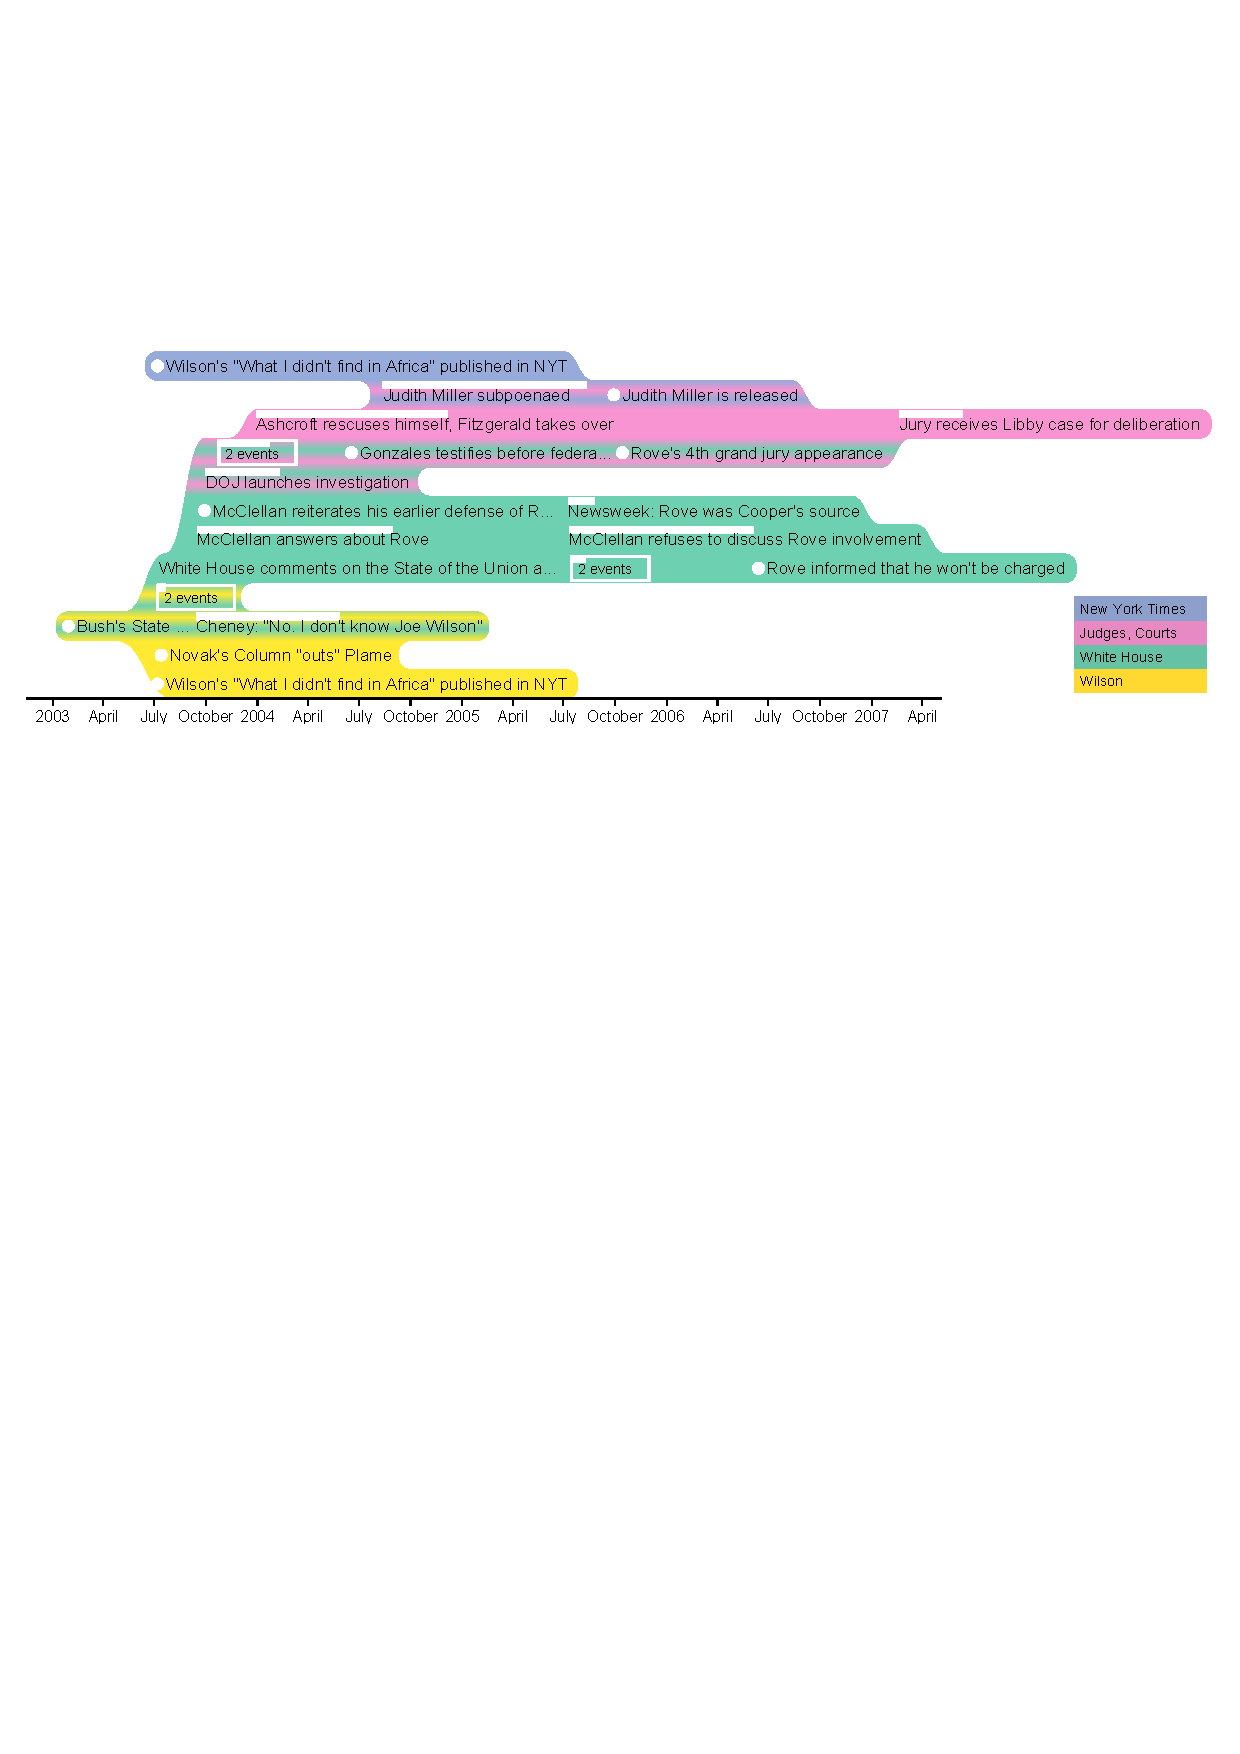
\includegraphics[width=120mm]{timesets}
};

\node (backtitle) [color=orange, yshift=170mm, font=\Large,  text width=140mm, align=center] at (79.5mm,0) {Visualization of Analytic Provenance for Sensemaking};

%\node [anchor=north west,inner sep=0] at (11mm, 92.25mm) (sensemap) {
%	\includegraphics[width=135mm]{sensemap-bw}
%};

\node [anchor=north west,inner sep=0] at (19mm, 97.25mm) (sm-browser) {
	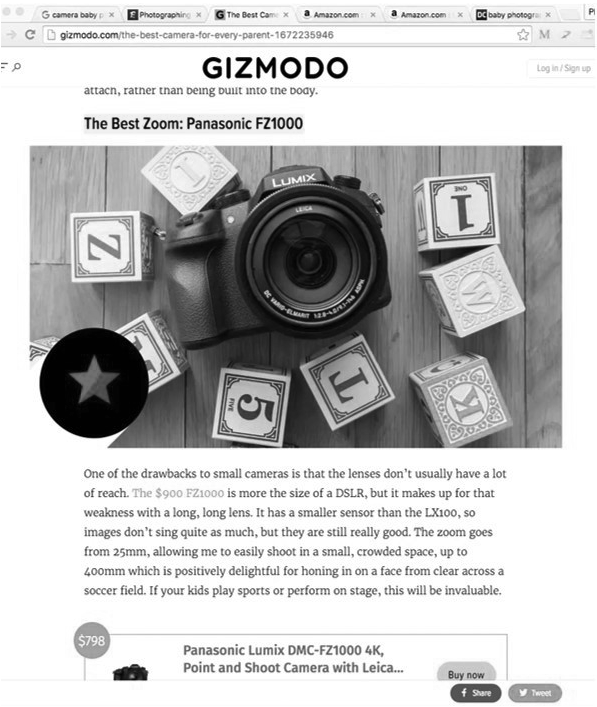
\includegraphics[width=70mm]{sm-browser}
};
%\node[below=1mm of sm-browser, color=orange, font=\sffamily\Large]{Browser Enhancement};

\node [right =0 of sm-browser,anchor=south west,yshift=-6.3mm] (sm-history) {
	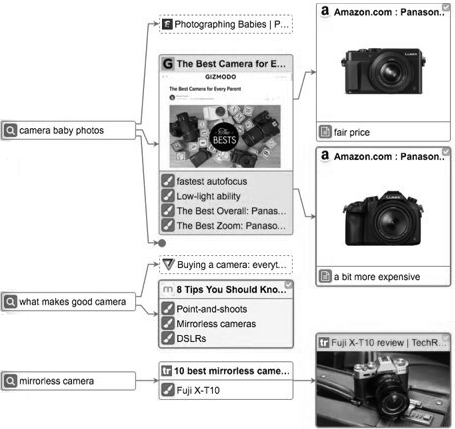
\includegraphics[width=49.5mm]{sm-history}
};
%\node[above=-2mm of sm-history, color=orange, font=\sffamily\Large]{History Map};

\node [below =-1mm of sm-history] (sm-knowledge) {
	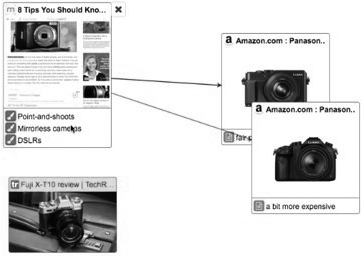
\includegraphics[width=49.5mm]{sm-knowledge}
};
%\node[below=0mm of sm-knowledge, color=orange, font=\sffamily\Large]{Knowledge Map};


\node (abstract) [color=white, below = 2mm of backtitle, text width=121mm, align=justify] {Sensemaking is an iterative and dynamic process, in which people collect data relevant to their tasks, analyze the collected information to produce new knowledge, and possibly inform further actions. During the sensemaking process, it is difficult for the human's working memory to keep track of the progress and to synthesize a large number of individual findings and derived hypotheses, thus limits the performance. Analytic provenance captures both the data exploration process and its accompanied reasoning, potentially addresses these information overload and disorientation problems. This thesis addresses the challenge of how to design interactive visualizations of analytic provenance data to support such an iterative and dynamic sensemaking. Its original contribution includes four visualizations that help users explore complex temporal and reasoning relationships hidden in the sensemaking problems, using both automatically and manually captured provenance. A deep understanding about the past could lighten the future.};

% spine
\node [rotate=-90,color=white, font=\Large] at (164.5mm,170mm) {Visualization of Analytic Provenance for Sensemaking};

\node [rotate=-90,color=white, font=\Large\sffamily] at (164.5mm,45mm) {Phong Hai Nguyen};

% shield on spine
\node [anchor=south west,inner sep=0] at (161mm, 10mm) (front) {
	
\includegraphics[height=8mm]{MdxShield}
};

\end{tikzpicture}

\end{document}